\subsubsection{Point sources}
\label{subsubsec:point_sources}
\index{Source type!point}
\index{Point source|see{Source type}}

\begin{figure}[!ht]
\centering
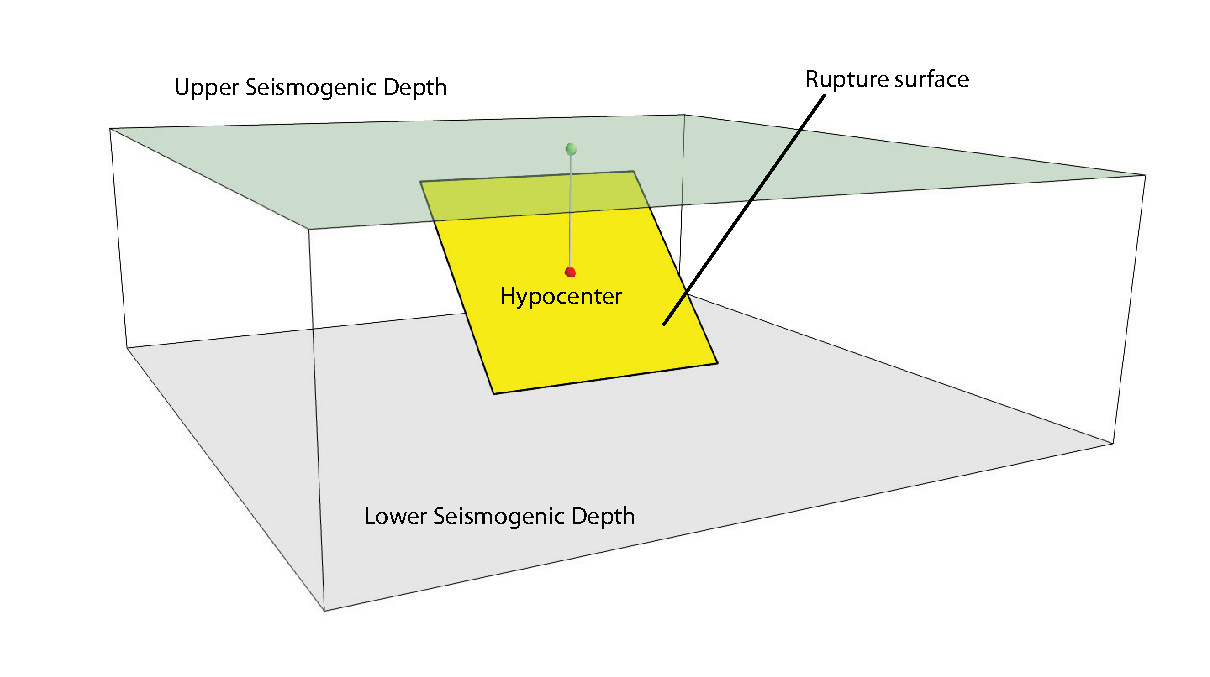
\includegraphics[width=10cm]{figures/hazard/single_rupture.pdf}
\caption{Single rupture}
\label{fig:single_rupture}
\end{figure}

The point source is the elemental source type adopted in the OpenQuake-engine
for modelling distributed seismicity. The \glsdesc{acr:oqe} always performs
calculations considering finite ruptures, even in the case of point sources.

These are the basic assumptions used to generate ruptures with point sources:

\begin{itemize}

    \item Ruptures have a rectangular shape

    \item Rupture hypocenter is located in the middle of the rupture

    \item Ruptures are limited at the top and at the bottom by two planes
    parallel to the topographic surface and placed at two characteristic
    depths named upper and lower seismogenic depths, respectively (see
    Figure~\ref{fig:single_rupture})

\end{itemize}

\paragraph{Source data}

For the definition of a point source the following parameters are required
(Figure~\ref{fig:single_rupture} shows some of the parameters described
below, together with an example of the surface of a generated rupture):

\begin{itemize}

    \item The coordinates of the point (i.e. longitude and latitude) [decimal
    degrees]

    \item The upper and lower seismogenic depths [km]

    \item One \gls{mfd}

    \item One magnitude-scaling relationship

    \item The rupture aspect ratio

    \item A distribution of nodal planes i.e. one (or several) instances
    of the following set of parameters:

    \begin{itemize}
        \item \gls{strike} [degrees]
        \item \gls{dip} [degrees]
        \item \gls{rake} [degrees]
    \end{itemize}

\item A magnitude independent depth distribution of hypocenters [km].

\end{itemize}

Figure~\ref{fig:point_source_multiple_ruptures} shows ruptures generated by a
point source for a range of magnitudes. Each rupture is centered on the
single hypocentral position admitted by this point source. Ruptures are
created by conserving the area computed using the specified magnitude-area
scaling relatioship and the corresponding value of magnitude.

\begin{figure}[ht!]
\centering
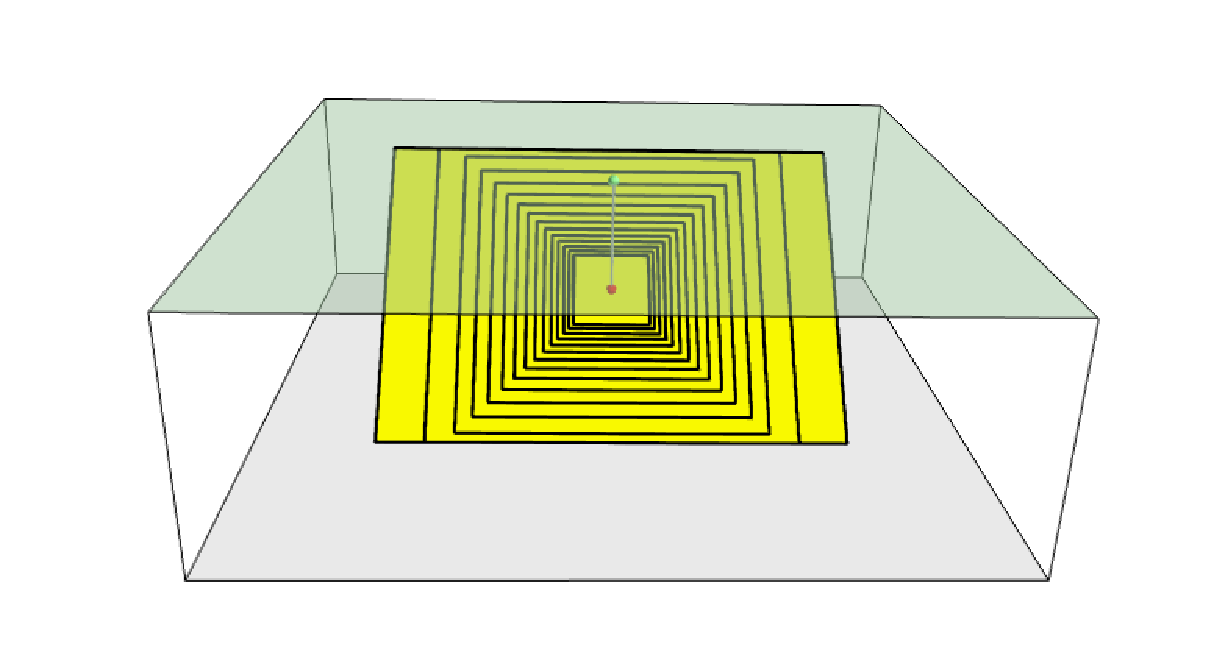
\includegraphics[width=10cm]{figures/hazard/point_source_multiple_ruptures.pdf}
\caption{Point source with multiple ruptures. Note the change in the aspect
ratio once the rupture width fills the entire seismogenic layer.}
\label{fig:point_source_multiple_ruptures}
\end{figure}

Below we provide the excerpt of an .xml file used to describe the properties of a point source. Note that in this example, ruptures occur on two possible nodal planes and two hypocentral depths. Figure~\ref{fig:point_source_ruptures} shows the ruptures generated by the point source.

\begin{listing}[htbp]
  \inputminted[firstline=1,firstnumber=1,fontsize=\footnotesize,frame=single,linenos,bgcolor=lightgray]{xml}{oqum/hazard/verbatim/input_point_source.xml}
  \caption{Example point source}
  \label{page:point_source_nrml}
\end{listing}

%The red part shows the the parameters used to describe the geometry of the point source, the blue part is the description of the magnitude-frequency distribution, the green text shows the nodal plane distribution and the text in magenta illustrates the hypocentral depth distribution.

%The text in black describes the parameters needed to generate the ruptures such as the \gls{msr} and the aspect ratio.



\begin{figure}[!ht]
\centering
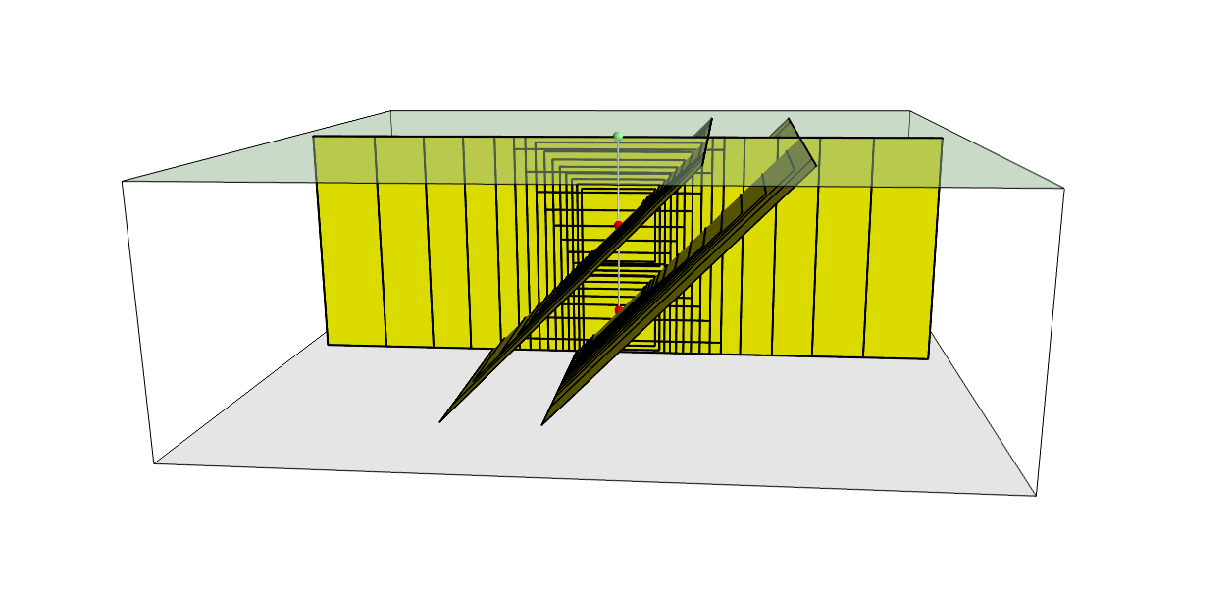
\includegraphics[width=10cm]{figures/hazard/pointsrc_2strike_2hypodep.pdf}
\caption{Ruptures produced by the source created using the information 
in the example .xml file described at page~\pageref{page:point_source_nrml}.}
\label{fig:point_source_ruptures}
\end{figure}

\subsubsection{Grid sources}
\label{subsubsec:grid_sources}
\index{Source type!grid}
\index{Grid source|see{Source type}}

A \gls{gridsource} is simply a collection of point sources distributed over a regular grid (usually equally spaced in longitude and latitude). In \gls{psha} a grid source can be considered a model alternative to area
sources, since they both model distributed seismicity. Grid sources are generally used to reproduce more faithfully the spatial pattern of seismicity depicted by the earthquakes occurred in the past; in
some models (e.g. \citet{petersen2008}) only events of low and intermediate magnitudes are considered. They are frequently, though not always, computed using seismicity smoothing algorithms \citep[][amongst many others]{frankel1995,woo1996}.

The use of smoothing algorithms to produce grid sources brings some
advantages compared to area sources, since (1) it removes most of the
unavoidable degree of subjectivity due to the definition of the geometries of the area sources and (2) it produces a spatial pattern of seismicity that is usually closer to what observed in the reality. Nevertheless, in many cases smoothing algorithms require an a-priori definition of some setup parameters that expose the calculation to a certain degree of partiality.

Grid sources are modeled in \gls{acr:oqe} simply as a set of point sources; in other words, a grid source is just a long list of point sources specified as described in the previous section (see page
\pageref{subsubsec:point_sources}).

\subsubsection{Area sources}
\label{subsubsec:area_sources}
\index{Source type!area}
\index{Area source|see{Source type}}

Area sources are usually adopted to describe the seismicity occurring over wide areas where the identification and characterization - i.e. the
unambiguous definition of position, geometry and seismicity occurrence
parameters - of single fault structures is difficult.

From a computation standpoint, area sources are comparable to grid sources since they are both represented in the engine by a list of point sources.

The \gls{acr:oqe} using the source data parameters (see below) creates an
equally spaced in distance grid of point sources where each point has the same seismicity occurrence properties (i.e. rate of events generated).

Below we provide a brief description of the parameters necessary to completely describe an area source.

\paragraph{Source data}

\begin{itemize}

    \item A polygon defining the external border of the area (i.e. a list of
    Longitude-Latitude [degrees] tuples) The current version of the OQ-engine doesn't
    support the definition of internal borders.

    \item The upper and lower seismogenic depths [km]

    \item One \gls{mfd}

    \item One \gls{msr}

    \item The rupture aspect ratio

    \item A distribution of nodal planes i.e. one (or several) instances of
    the following set of parameters

    \begin{itemize}
        \item \gls{strike} [degrees]
        \item \gls{dip} [degrees]
        \item \gls{rake} [degrees]
    \end{itemize}

    \item A magnitude independent depth distribution of hypocenters [km].

\end{itemize}

Below we provide the excerpt of an .xml file used to describe the properties of an area source. The ruptures generated by the area source described in the example are controlled by two nodal planes and have hypocenters at localized at two distinct depths.

\begin{listing}[htbp]
  \inputminted[firstline=1,firstnumber=1,fontsize=\footnotesize,frame=single,linenos,bgcolor=lightgray]{xml}{oqum/hazard/verbatim/input_area_source.xml}
  \caption{Example area source}
  \label{lst:area_source}
\end{listing}

%The red text describes the parameters used to describe the geometry of the area source; the blue part is the description of the magnitude-frequency distribution; the green text displays the nodal plane distribution; and the text in magenta illustrates the hypocentral depth distribution.

%The text in gray describes the parameters required to generate the ruptures such as the \gls{msr} and the aspect ratio.

